\subsection{Insegnante}

\subsubsection{Panoramica insegnante}
\begin{comment}
\begin{figure}[H]
\centering
\includegraphics[width=17cm, height=20cm]{img/} 
\caption{Panoramica insegnante}
\end{figure}
\end{comment}


\subsubsection{UC 2.1 - Visualizzazione della dashboard}
\begin{itemize}
	\item[•] \textbf{Attori}: Insegnante;
	\item[•] \textbf{Descrizione}: l’insegnante accede alla propria dashboard;
	\item[•] \textbf{Precondizione}: l'insegnante si è autenticato;
	\item[•] \textbf{Postcondizione}: l'insegnante visualizza tutti i componenti della sua dashboard;
	\item[•] \textbf{Flusso degli eventi}: l’insegnante ha effettuato il login e viene reindirizzato alla propria dashboard.
\end{itemize}

\subsubsection{UC 2.2 - Inserimento di un nuovo esercizio}

\begin{comment}
\begin{figure}[H]
	\centering
	\includegraphics[width=17cm]{img/} 
	\caption{Caso d'uso UC 2.2;}
\end{figure}
\end{comment}

\begin{itemize}
	\item[•] \textbf{Attori}: Insegnante;
	\item[•] \textbf{Descrizione}: l'insegnante aggiunge un nuovo esercizio. 
	\item[•] \textbf{Precondizione}: l'insegnante si è autenticato e visualizza la propria dashboard;
	\item[•] \textbf{Postcondizione}: l'insegnante ha inserito un esercizio;
	\item[•] \textbf{Flusso degli eventi}:
	\begin{enumerate}
		\item UC 2.2.1 - Selezione lingua esercizio;
		\item UC 2.2.2 - Inserimento testo esercizio;
		\item UC 2.2.3 - Visualizzazione analisi automatica;
		\item UC 2.2.5 - Modifica tag automatico;
		\item UC 2.2.6 - Modifica visibilità esercizio;
		\item UC 2.2.7 - Visualizzazione errori sintassi testo;
		\item UC 2.2.8 - Assegna esercizio;
		\item UC 2.2.9 - Conferma aggiunta esercizio.
	\end{enumerate}
	\item[•] \textbf{Estensioni}:	
	\begin{enumerate}
		\item UC 2.2.7.1 - Interruzione inserimento esercizio.
	\end{enumerate}
	\item[•] \textbf{Flusso degli eventi alternativo}:
	\begin{enumerate}
		\item UC 2.2.4 - Inserimento soluzione alternativa.
	\end{enumerate}
\end{itemize}


\subsubsection{UC 2.2.1 - Selezione lingua esercizio}
\begin{itemize}
	\item[•] \textbf{Attori}: Insegnante;
	\item[•] \textbf{Descrizione}: l'insegnante sceglie la lingua dell'esercizio che vuole scrivere;
	\item[•] \textbf{Precondizione}: l'insegnante sta inserendo un esercizio;
	\item[•] \textbf{Postcondizione}: l'insegnante ha scelto la lingua dell'esercizio;
	\item[•] \textbf{Flusso degli eventi}: l'insegnante durante l'inserimento di un esercizio sceglie la lingua dell'esercizio.
\end{itemize}

\subsubsection{UC 2.2.2 - Inserimento testo esercizio}
\begin{itemize}
	\item[•] \textbf{Attori}: Insegnante;
	\item[•] \textbf{Descrizione}: l'insegnante scrive il testo dell'esercizio;
	\item[•] \textbf{Precondizione}: l'insegnante sta inserendo un esercizio;
	\item[•] \textbf{Postcondizione}: l'insegnante ha inserito il testo dell'esercizio;
	\item[•] \textbf{Flusso degli eventi}: l'insegnante durante l'inserimento di un esercizio scrive il testo dell'esercizio.
\end{itemize}

\subsubsection{UC 2.2.3 - Visualizzazione analisi automatica} DA FARE

\subsubsection{UC 2.2.4 - Inserimento soluzione alternativa}
\begin{itemize}
	\item[•] \textbf{Attori}: Insegnante;
	\item[•] \textbf{Descrizione}: l'insegnante può inserire una soluzione alternativa;
	\item[•] \textbf{Precondizione}: l'insegnante visualizza la soluzione dell'esercizio;
	\item[•] \textbf{Postcondizione}: l'insegnante aggiunge una soluzione alternativa;
	\item[•] \textbf{Flusso degli eventi}: l'insegnante durante l'inserimento di un esercizio, in caso di esercizi con più soluzioni, inserisce tag alternativi all'esercizio;
\end{itemize}


\subsubsection{UC 2.2.5 - Modifica tag automatico}
\begin{itemize}
	\item[•] \textbf{Attori}: Insegnante;
	\item[•] \textbf{Descrizione}: l'insegnante modifica il tag generato automaticamente;
	\item[•] \textbf{Precondizione}: l'insegnante visualizza la soluzione dell'esercizio;
	\item[•] \textbf{Postcondizione}: l'insegnante ha modificato i tag generati automaticamente;
\item[•] \textbf{Flusso degli eventi}:
\begin{enumerate}
		\item Selezione tag da modificare;
		\item Selezione tag corretto.
\end{enumerate}
	
\end{itemize}

\subsubsection{UC 2.2.6 - Modifica visibilità esercizio}
\begin{itemize}
	\item[•] \textbf{Attori}: Insegnante;
	\item[•] \textbf{Descrizione}: l'insegnante imposta la visibilità dell'esercizio, ovvero quali allievi o classi possono visualizzarlo e sceglierlo;
	\item[•] \textbf{Precondizione}: l'insegnante sta inserendo un esercizio;
	\item[•] \textbf{Postcondizione}: l'insegnante ha modificato la visibilità dell'esercizio;
	\item[•] \textbf{Flusso degli eventi}: l'insegnante sceglie (tra le visibilità proposte) che visibilità dare all'esercizio.
\end{itemize}

\subsubsection{UC 2.2.7 - Visualizzazione errori sintassi testo}
\begin{itemize}
	\item[•] \textbf{Attori}: Insegnante;
	\item[•] \textbf{Descrizione}: l'insegnante visualizza gli errori relativi alla sintassi e la forma del testo che ha inserito;
	\item[•] \textbf{Precondizione}: l'insegnante sta inserendo un esercizio;
	\item[•] \textbf{Postcondizione}: l'insegnante visualizza gli errori relativi al testo inserito;
	\item[•] \textbf{Flusso degli eventi}: l'insegnante durante l'inserimento del testo, commette un errore di sintassi.
\end{itemize}

\subsubsection{UC 2.2.7.1 - Interruzione inserimento esercizio} DA FARE

\subsubsection{UC 2.2.8 - Assegna esercizio} DA FARE
\begin{itemize}
	\item[•] \textbf{Attori}: Insegnante;
	\item[•] \textbf{Descrizione}:;
	\item[•] \textbf{Precondizione}:;
	\item[•] \textbf{Postcondizione}:;
	\item[•] \textbf{Flusso degli eventi}: .
\end{itemize}

\subsubsection{UC 2.2.9 - Conferma aggiunta esercizio}
\begin{itemize}
	\item[•] \textbf{Attori}: Insegnante;
	\item[•] \textbf{Descrizione}: l'insegnante aggiunge un esercizio al sistema;
	\item[•] \textbf{Precondizione}: l'insegnante sta inserendo un esercizio;
	\item[•] \textbf{Postcondizione}: l'insegnante conferma l'inserimento dell'esercizio;
	\item[•] \textbf{Flusso degli eventi}:l'insegnante ha completato e selezionato tutti i campi presenti ed ha confermato l'aggiunta dell'esercizio.
\end{itemize}



\subsubsection{UC 2.3 - Visualizzazione storico frasi inserite}
\begin{itemize}
	\item[•] \textbf{Attori}: Insegnante	   
	\item[•] \textbf{Descrizione}: l'insegnante visualizza lo storico delle frasi inserite sotto forma tabellare; 
	\item[•] \textbf{Precondizione}: l'insegnante sta visualizzando la propria dashboard;
	\item[•] \textbf{Postcondizione}: l'insegnante naviga all’interno della lista di frasi che ha inserito;
	\item[•] \textbf{Flusso degli eventi}: l'insegnante seleziona apposito campo per la visualizzazione dello storico frasi inserite.
\end{itemize}


\subsubsection{UC 2.3.1 - Visualizzazione dettaglio esercizio}
\begin{itemize}
	\item[•] \textbf{Attori}: Insegnante;
	\item[•] \textbf{Descrizione}: l'insegnante seleziona dalla lista degli esercizi assegnati un esercizio e ne visualizza i dettagli: nome e cognome dell'allievo che ha svolto l'esercizio ;
	\item[•] \textbf{Precondizione}: l'insegnante visualizza la lista di frasi che ha inserito;
	\item[•] \textbf{Postcondizione}: l'insegnante visualizza i dettagli di un esercizio inserito;
	\item[•] \textbf{Flusso degli eventi}: l'insegnante naviga all'interno della lista di frasi che ha inserito e seleziona un esercizio specifico.
\end{itemize}


\subsubsection{UC 2.4 - Visualizzazione esercizi svolti dagli allievi}
\begin{itemize}
	\item[•] \textbf{Attori}: Insegnante;
	\item[•] \textbf{Descrizione}:  l'insegnante visualizza l'elenco degli esercizi svolti dagli allievi;
	\item[•] \textbf{Precondizione}: l'insegnante visualizza la propria dashboard;
	\item[•] \textbf{Postcondizione}: l'insegnante naviga all'interno della lista di esercizi svolti;
	\item[•] \textbf{Flusso degli eventi}: l'insegnante seleziona apposito campo per la visualizzazione degli esercizi svolti dai propri allievi.
\end{itemize}

\subsubsection{UC 2.5 - Visualizzazione dei propri allievi}
\begin{itemize}
	\item[•] \textbf{Attori}: Insegnante;
	\item[•] \textbf{Descrizione}: l'insegnante visualizza la lista dei suoi allievi: nome, cognome, data di nascita, classe di appartenenza, insegnante preferito;
	\item[•] \textbf{Precondizione}: l'insegnante visualizza la propria dashboard;
	\item[•] \textbf{Postcondizione}: l'insegnante visualizza la lista dei propri allievi.
	\item[•] \textbf{Flusso degli eventi}:  l'insegnante seleziona l'apposito campo per la visualizzazione della lista dei propri allievi.
\end{itemize}


\subsubsection{UC 2.6 - Modifica esercizio}


\begin{comment}
\begin{figure}[H]
\centering
\includegraphics[width=17cm]{img/} 
\caption{Caso d'uso UC 2.6}
\end{figure}
\end{comment}

\begin{itemize}
	\item[•] \textbf{Attori}: Insegnante;
	\item[•] \textbf{Descrizione}: l'insegnante può modificare il testo, la visibilità, i tag, le soluzioni alternative e può riassegnare un esercizio precedentemente inserito;
	\item[•] \textbf{Precondizione}: l'insegnante visualizza lo storico delle frasi inserite;
	\item[•] \textbf{Postcondizione}: l'insegnante ha modificato l'esercizio;
	\item[•] \textbf{Flusso degli eventi}:
	\begin{enumerate}
		\item Selezione procedura modifica esercizio;
		\item UC 2.6.1 - Modifica testo esercizio;
		\item UC 2.6.2 - Modifica tag automatico;
		\item UC 2.6.3 - Modifica visibilità;
		\item UC 2.6.4 - Riassegnazione esercizio;
		\item UC 2.6.5 - Eliminazione soluzione alternativa;
		\item UC 2.6.6 - Salvataggio modifiche.
	\end{enumerate}
	\item[•] \textbf{Estensioni}:	
	\begin{enumerate}
		\item UC 2.6.7 - Annullamento modifiche.
	\end{enumerate}
\end{itemize}


\subsubsection{UC 2.6.1 - Modifica testo esercizio} DA FARE
\subsubsection{UC 2.6.2 - Modifica tag automatico} DA FARE
\subsubsection{UC 2.6.3 - Modifica visibilità} DA FARE
\subsubsection{UC 2.6.4 - Riassegnazione esercizio} DA FARE

\subsubsection{UC 2.6.5 - Eliminazione soluzione alternativa}
\begin{itemize}
	\item[•] \textbf{Attori}: Insegnante;
	\item[•] \textbf{Descrizione}: l'insegnante elimina una delle soluzioni alternative inserite in precedenza;
	\item[•] \textbf{Precondizione}: l'insegnante sta modificando un esercizio;
	\item[•] \textbf{Postcondizione}: l'insegnante ha eliminato una soluzione alternativa di un esercizio.
	\item[•] \textbf{Flusso degli eventi}: l'insegnante seleziona apposito campo per l'eliminazione della soluzione alternativa.
\end{itemize}

\subsubsection{UC 2.6.6 - Salvataggio modifiche} DA FARE

\subsubsection{UC 2.6.7 - Annullamento modifiche}
\begin{itemize}
	\item[•] \textbf{Attori}: Insegnante;
	\item[•] \textbf{Descrizione}: l'insegnante annulla le modifiche inserite all'interno di un esercizio; 
	\item[•] \textbf{Precondizione}: l'insegnante sta modificando un esercizio;
	\item[•] \textbf{Postcondizione}: l'esercizio non è modificato.
	\item[•] \textbf{Flusso degli eventi}:l'insegnante interrompe la procedura di modifica.
\end{itemize}

\subsubsection{UC 2.7 - Eliminazione esercizio}
\begin{itemize}
	\item[•] \textbf{Attori}: Insegnante;
	\item[•] \textbf{Descrizione}: l'insegnante ha la possibilità di eliminare un esercizio precedentemente inserito;
	\item[•] \textbf{Precondizione}: l'insegnante visualizza lo storico delle frasi inserite;
	\item[•] \textbf{Postcondizione}: l'insegnante ha eliminato l'esercizio precedentemente inserito;
	\item[•] \textbf{Flusso degli eventi}:l'insegnante seleziona un esercizio specifico e seleziona apposito campo per l'eliminazione.
\end{itemize}

\subsubsection{UC 2.2.9 - Salvataggio modifiche}
\begin{itemize}
	\item[•] \textbf{Attori}: Insegnante;
	\item[•] \textbf{Descrizione}: l'insegnante salva l'esercizio e le possibili modifiche;
	\item[•] \textbf{Precondizione}: l'insegnante sta inserendo un esercizio;
	\item[•] \textbf{Postcondizione}: l'insegnante ha salvato l'esercizio;
	\item[•] \textbf{Flusso degli eventi}:l'insegnante ha completato e selezionato tutti i campi presenti.
\end{itemize}

\subsubsection{UC 2.8 - Modifica dati utente}
\begin{itemize}
	\item[•] \textbf{Attori}: Insegnante;
	\item[•] \textbf{Descrizione}: l'insegnante modifica i propri dati personali, cioè tutti i dati inseriti in fase di registrazione;
	\item[•] \textbf{Precondizione}: l'insegnante visualizza la propria dashboard;
	\item[•] \textbf{Postcondizione}: l'insegnante ha modificato uno o più dati personali;
	\item[•] \textbf{Flusso degli eventi}:
	\begin{enumerate}
		\item Selezione procedura modifica dati personali;
		\item UC 2.8.1 - Modifica email ;
		\item UC 2.8.2 - Modifica nome;
		\item UC 2.8.3 - Modifica cognome;
		\item UC 2.8.4 - Modifica password
		\item UC 2.8.5 - Modifica data di nascita;
		\item UC 2.8.6 - Modifica lingua interfaccia applicativo;
		\item UC 2.8.7 - Conferma modifica dati.
	\end{enumerate}
\end{itemize}

\subsubsection{UC 2.8 Modifica dati utente}  DA FARE
\subsubsection{UC 2.8.1 - Modifica email}   DA FARE
\subsubsection{UC 2.8.2 - Modifica nome}  DA FARE
\subsubsection{UC 2.8.3 - Modifica cognome}  DA FARE


\subsubsection{UC 2.8.4 - Modifica password}  DA FARE
	\subsubsection{UC 2.8.4.1 Inserimento nuova Password}  DA FARE
	\subsubsection{UC 2.8.4.2 Inserimento conferma nuova password}  DA FARE
	
	
\subsubsection{UC 2.8.5 - Modifica data di nascita}  DA FARE
\subsubsection{UC 2.8.6 Modifica lingua interfaccia applicativo}  DA FARE
\subsubsection{UC 2.8.7 - Conferma modifica dati}  DA FARE




\subsubsection{UC 2.9 - Visualizzazione elenco classi}
\begin{itemize}
	\item[•] \textbf{Attori}: Insegnante;
	\item[•] \textbf{Descrizione}: l'insegnante può modificare i propri dati utente;
	\item[•] \textbf{Precondizione}: l'insegnante è stato autenticato dal sistema;
	\item[•] \textbf{Postcondizione}: l'insegnante ha modificato i propri dati personali;
	\item[•] \textbf{Flusso degli eventi}:l'insegnante seleziona l'apposito campo per la visualizzazione della lista classi.
\end{itemize}

\subsubsection{UC 2.9.1 - Crea nuova classe}
\begin{figure}[H]
	\centering
	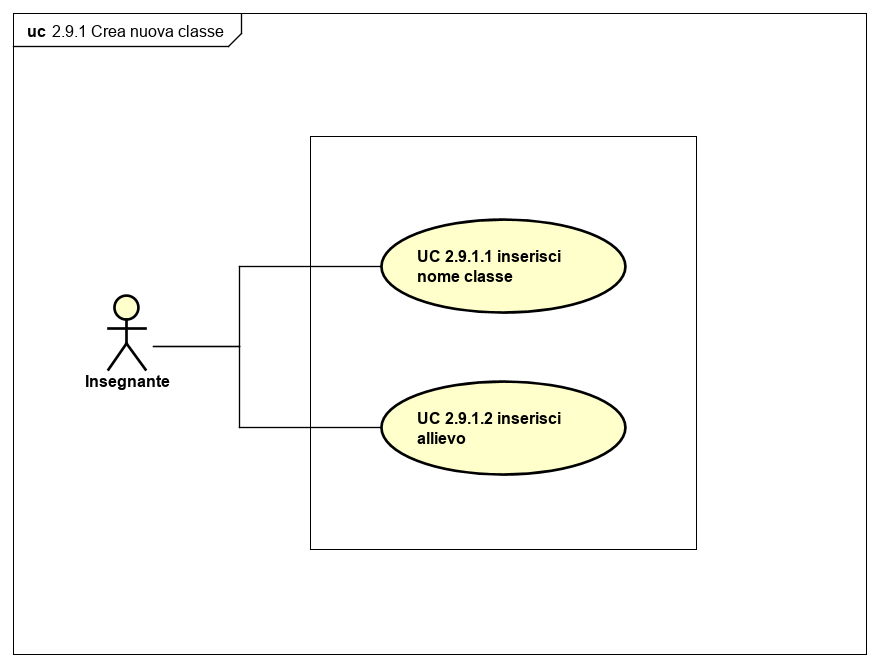
\includegraphics[width=17cm]{img/Crea_nuova_classe.png} 
	\caption{Caso d'uso UC 2.9.1;}
\end{figure}

\begin{itemize}
	\item[•] \textbf{Attori}: Insegnante;
	\item[•] \textbf{Descrizione}: l'insegnante può modificare i propri dati utente;
	\item[•] \textbf{Precondizione}: l'insegnante è stato autenticato dal sistema;
	\item[•] \textbf{Postcondizione}: l'insegnante ha modificato i propri dati personali;
	\item[•] \textbf{Flusso degli eventi}:
	\begin{enumerate}
		\item UC 2.9.1.1 inserisci nome classe;
		\item UC 2.9.1.2 inserisci allievo.
	\end{enumerate}
	\item[•] \textbf{Flusso degli eventi alternativo}:
	\begin{enumerate}
		\item UC 2.9.1.3 rimuovi allievo
	\end{enumerate}
\end{itemize}

\begin{figure}[H]
	\centering
	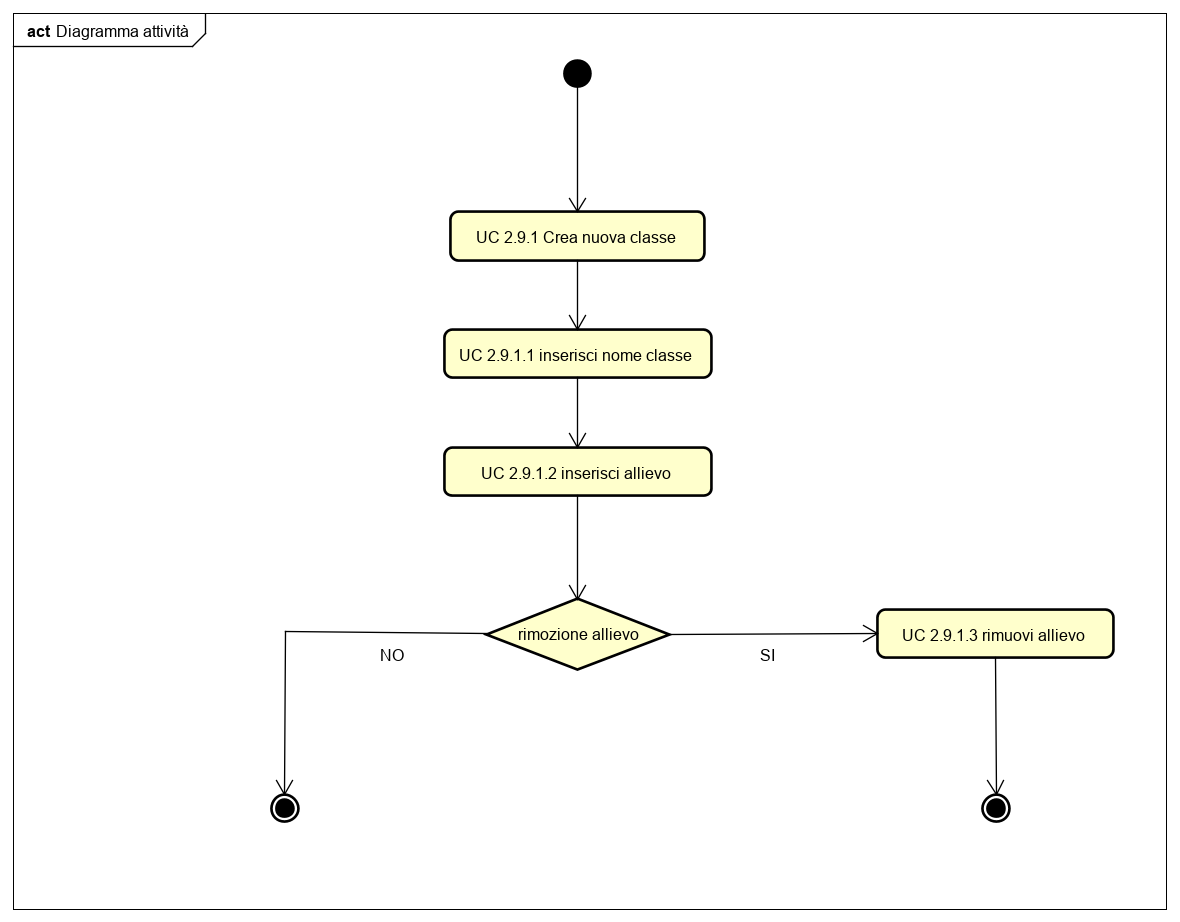
\includegraphics[width=17cm]{img/Diagramma_attivita_crea_classe.png} 
	\caption{Diagramma attività UC 2.9.1;}
\end{figure}


\subsubsection{UC 2.9.1.1 inserisci nome classe}  DA FARE
\subsubsection{UC 2.9.1.2 inserisci allievo}  DA FARE
\subsubsection{UC 2.9.1.3 rimuovi allievo}  DA FARE


\subsubsection{UC 2.9.2 modifica classe}  DA FARE
\begin{itemize}
	\item[•] \textbf{Attori}: Insegnante;
	\item[•] \textbf{Descrizione}: ;
	\item[•] \textbf{Precondizione}: ;
	\item[•] \textbf{Postcondizione}: ;
	\item[•] \textbf{Flusso degli eventi}:
	\begin{enumerate}
		\item UC 2.9.2.1 modifica nome classe;
		\item UC 2.9.2.2 inserisci allievo;
	\end{enumerate}
	\item[•] \textbf{Flusso degli eventi alternativo}:
	\begin{enumerate}
		\item UC 2.9.2.3 rimuovi allievo
	\end{enumerate}
\end{itemize}

	\subsubsection{UC 2.9.2.1 modifica nome classe}  DA FARE
	\subsubsection{UC 2.9.2.2 inserisci allievo}  DA FARE
	\subsubsection{UC 2.9.2.3 rimuovi allievo}  DA FARE


\subsubsection{UC 2.9.3 elimina classe}  DA FARE